\documentclass[ManualeUtente]{subfiles}

\begin{document}
	
	\chapter{University}
	After logging as university user, you will see this screen:
	\begin{figure}[H]
		\centering
		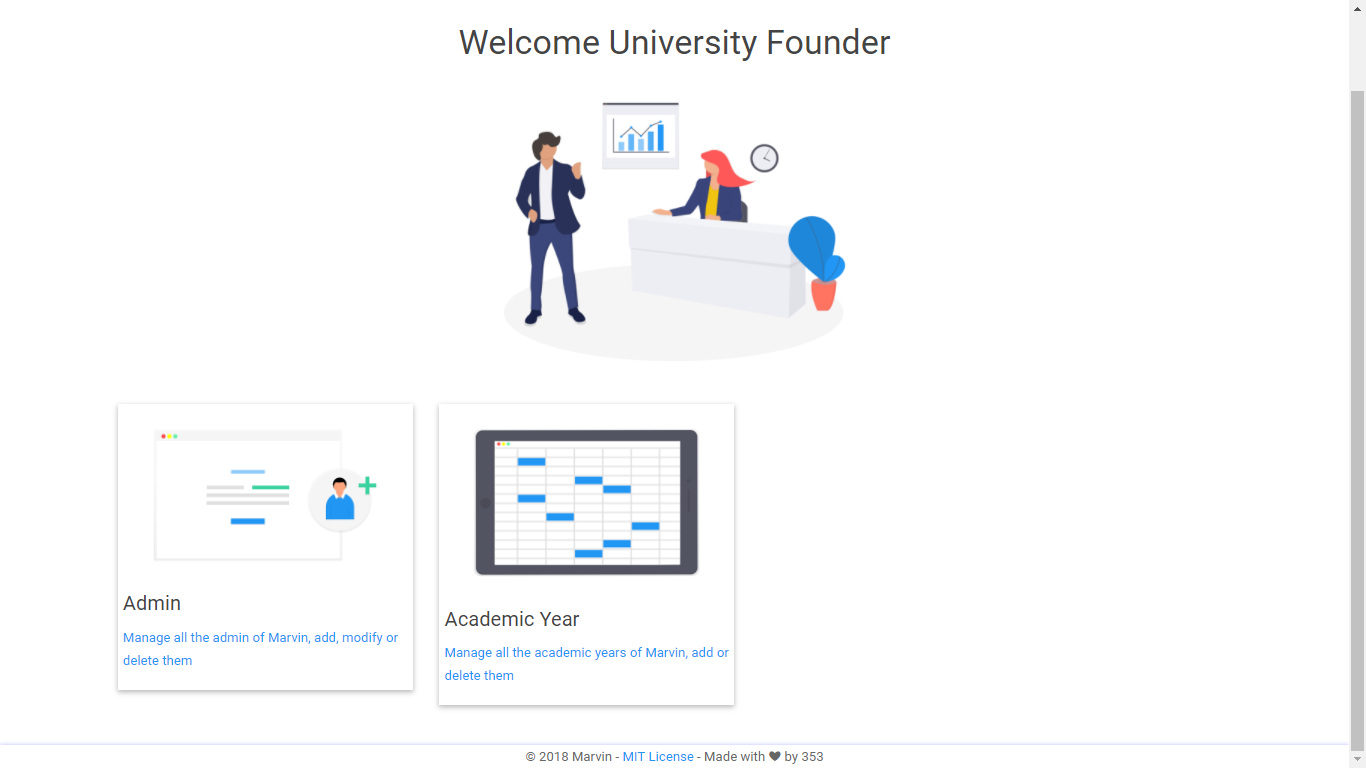
\includegraphics[width=0.7\linewidth]{./image/University}
		\caption[University]{University home page}
		\label{fig:university1}
	\end{figure}
	\newpage
	\section{Admins management}
	To manage admins, you have to click on the right section\\
	\begin{figure}[H]
		\centering
		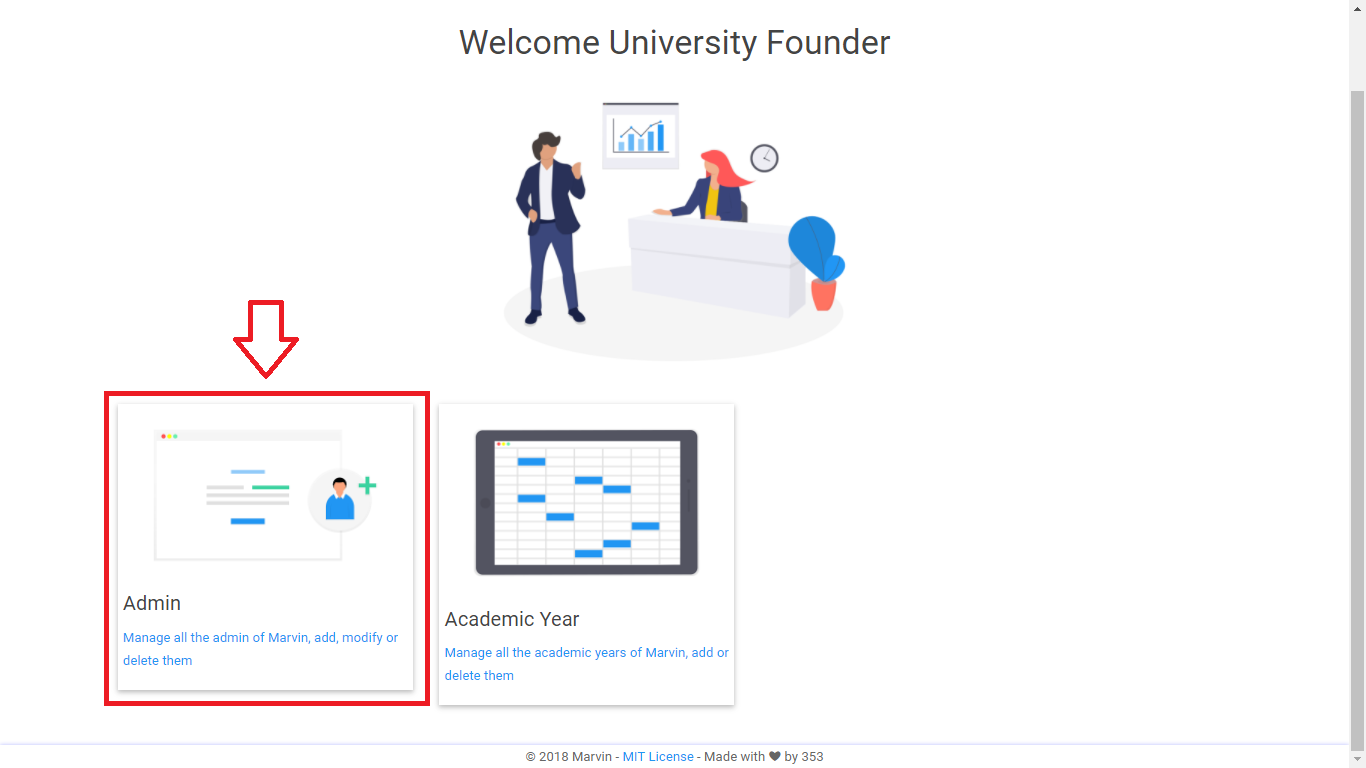
\includegraphics[width=0.7\linewidth]{./image/UniAdmin}
		\caption[Manage admin]{Manage admins}
		\label{fig:uniadmin}
	\end{figure}
	
	\subsection{Add a new admin}
	\begin{figure}[H]
		\centering
		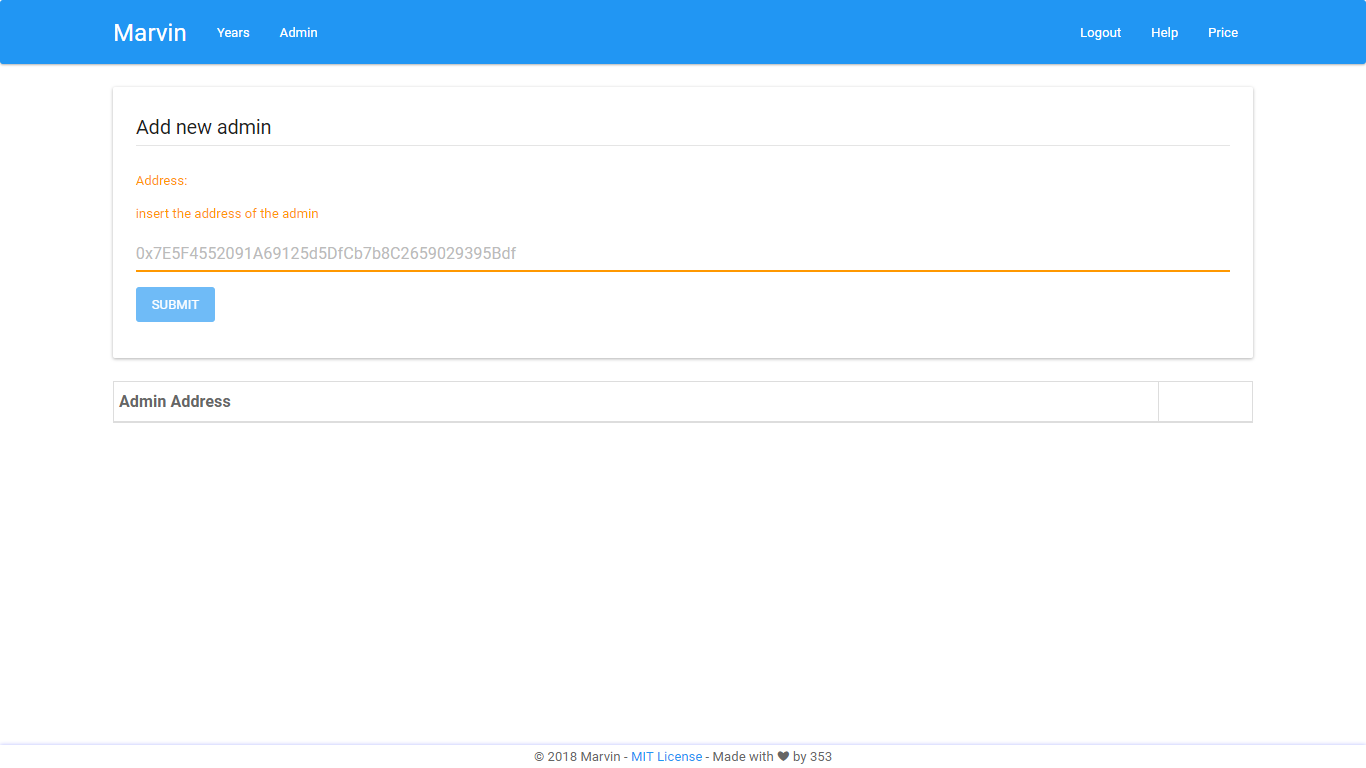
\includegraphics[width=0.7\linewidth]{image/UniversityAddAmin}
		\caption[Add admin]{Add a new admin}
		\label{fig:Add a new admin}
	\end{figure}\newpage
	To add a new admin, you have to go to the manage admins section and:
	\begin{enumerate}
		\item Insert the admin's public address in the form;
		\begin{figure}[H]
			\centering
			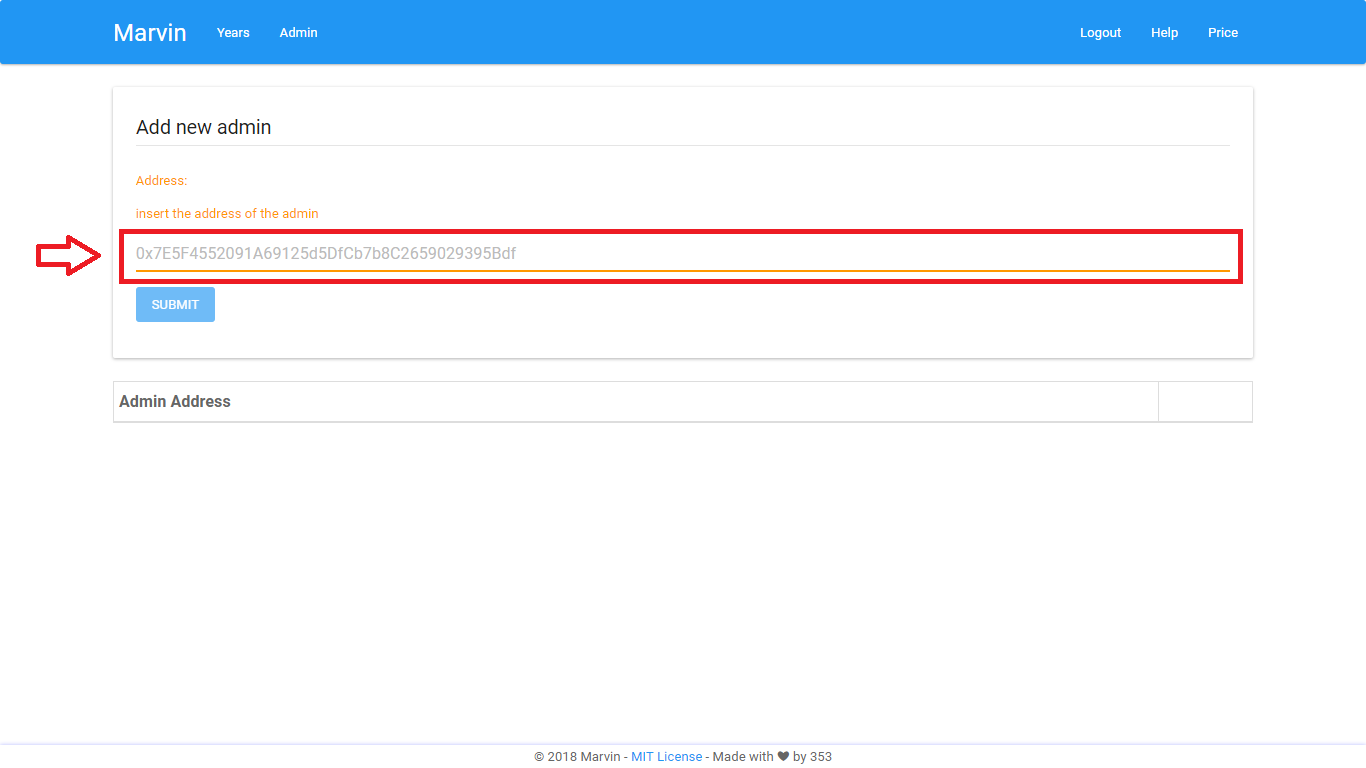
\includegraphics[width=0.7\linewidth]{image/UniversityAddAmin1}
			\caption[Add admin form]{Fill the form}
			\label{fig:Add a new admin, fill the form}
		\end{figure}
		\item And then click the button ``SUBMIT".
		\begin{figure}[H]
			\centering
			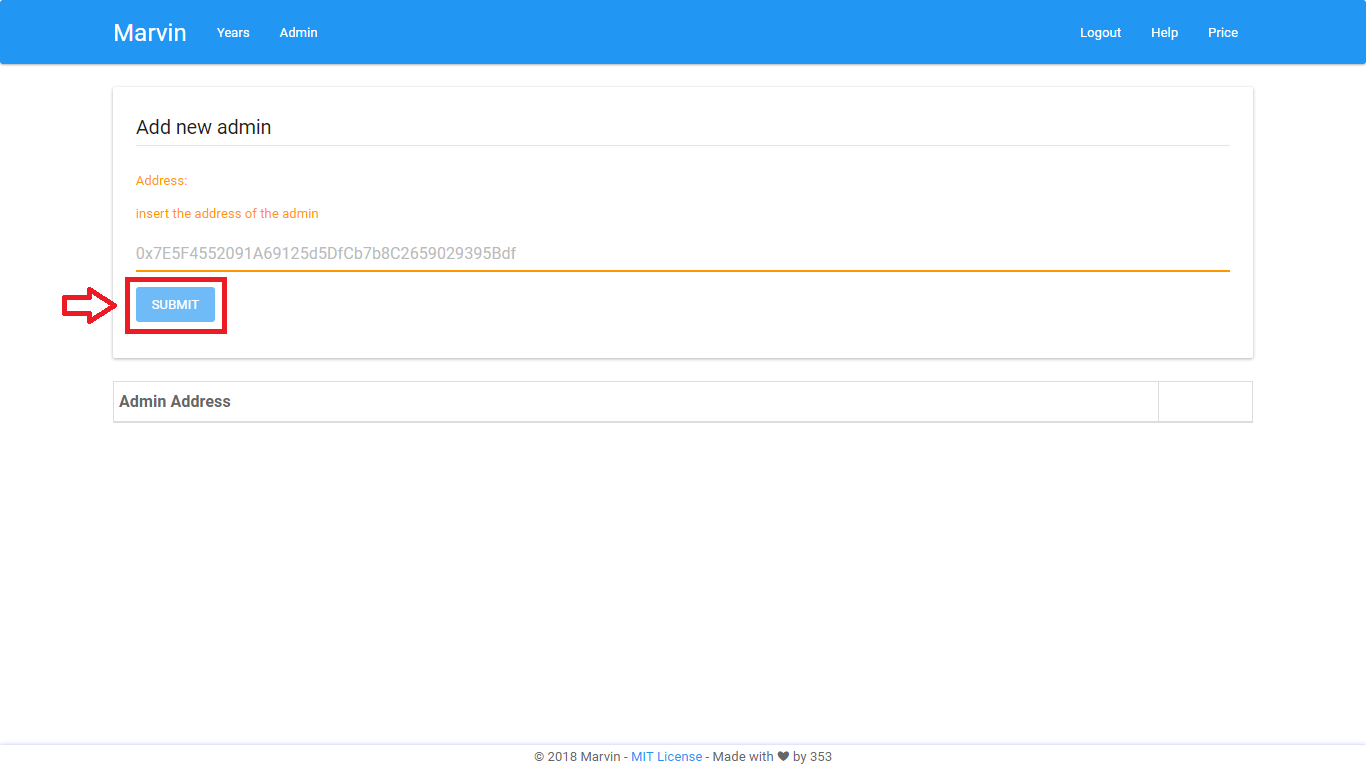
\includegraphics[width=0.7\linewidth]{image/UniversityAddAmin2}
			\caption[Add admin submit]{Click submit}
			\label{fig:Add a new admin, click submit}
		\end{figure}
	\end{enumerate}
	\newpage
	\subsection{Remove an admin}
	To remove an admin click the ``DELETE" button next to the admin you want to delete.
	\begin{figure}[H]
		\centering
		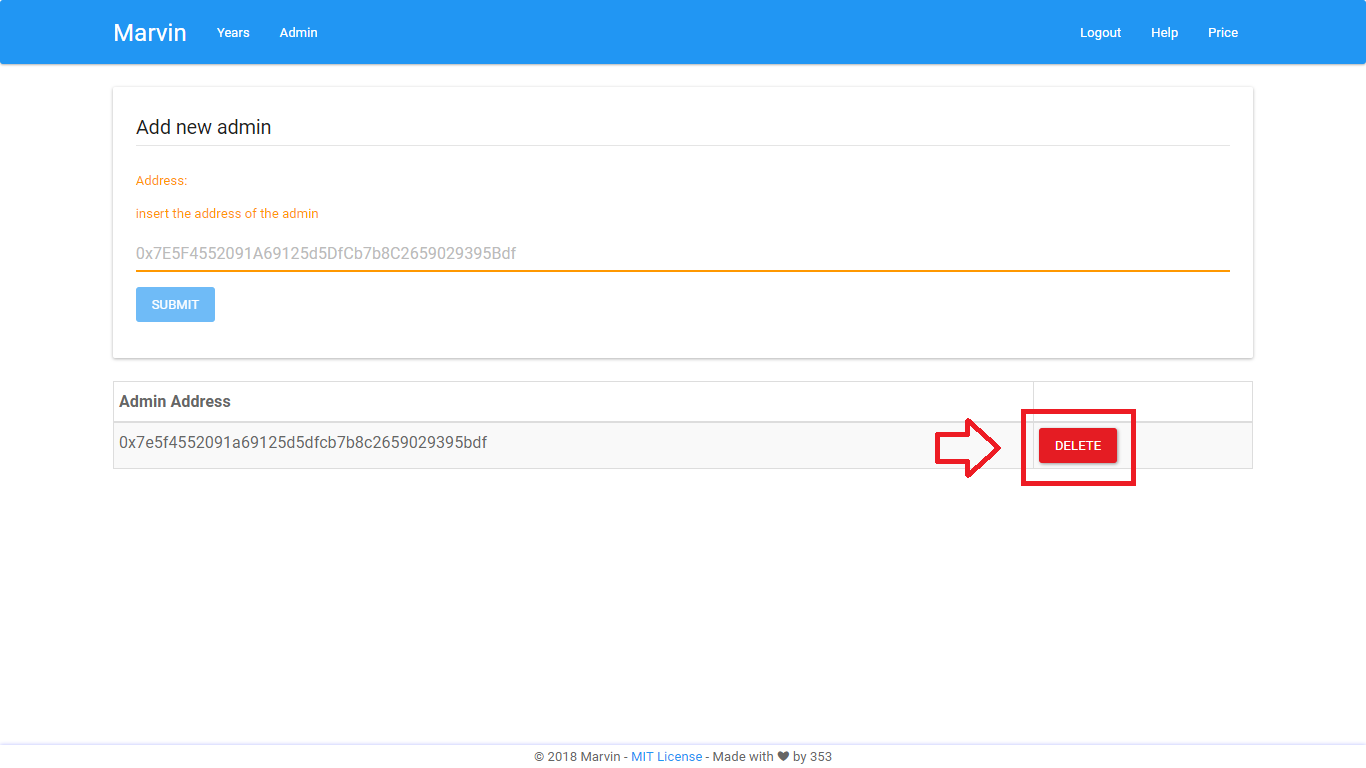
\includegraphics[width=0.7\linewidth]{image/DeleteAdmin}
		\caption[Delete admin]{Delete an admin}
		\label{fig:Delete an admin}
	\end{figure}
	\newpage
	
	\section{Academic years management}
	To manage academic years, you have to click on the right section.
	\begin{figure}[H]
		\centering
		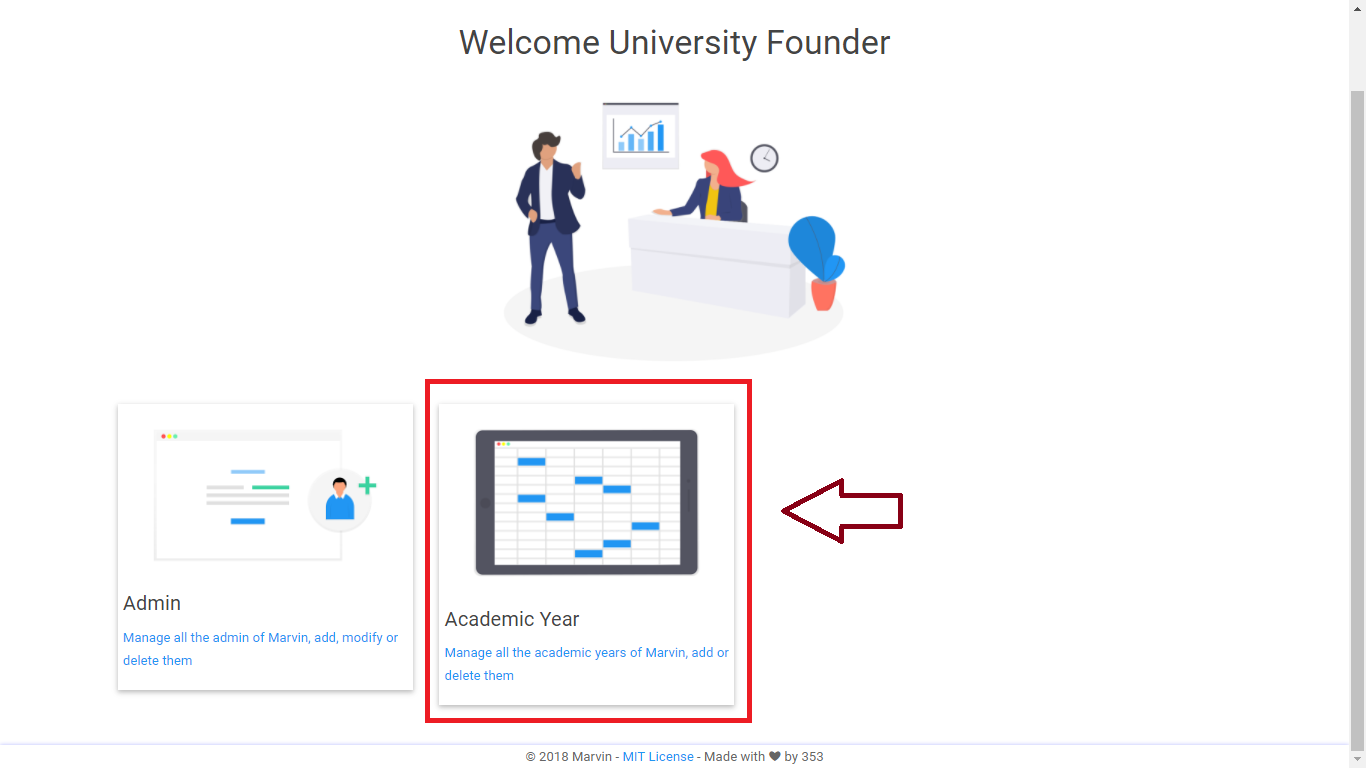
\includegraphics[width=0.7\linewidth]{image/UniAcademicYear}
		\caption[Add year]{Add a new academic year}
		\label{fig:Add a new academic year}
	\end{figure}
	\subsection{Add a new academic year}
	To add a new academic year, you must go to the manage academic years' section and:
	\begin{enumerate}
		\item Insert the year you want to add in the form;
		\begin{figure}[H]
			\centering
			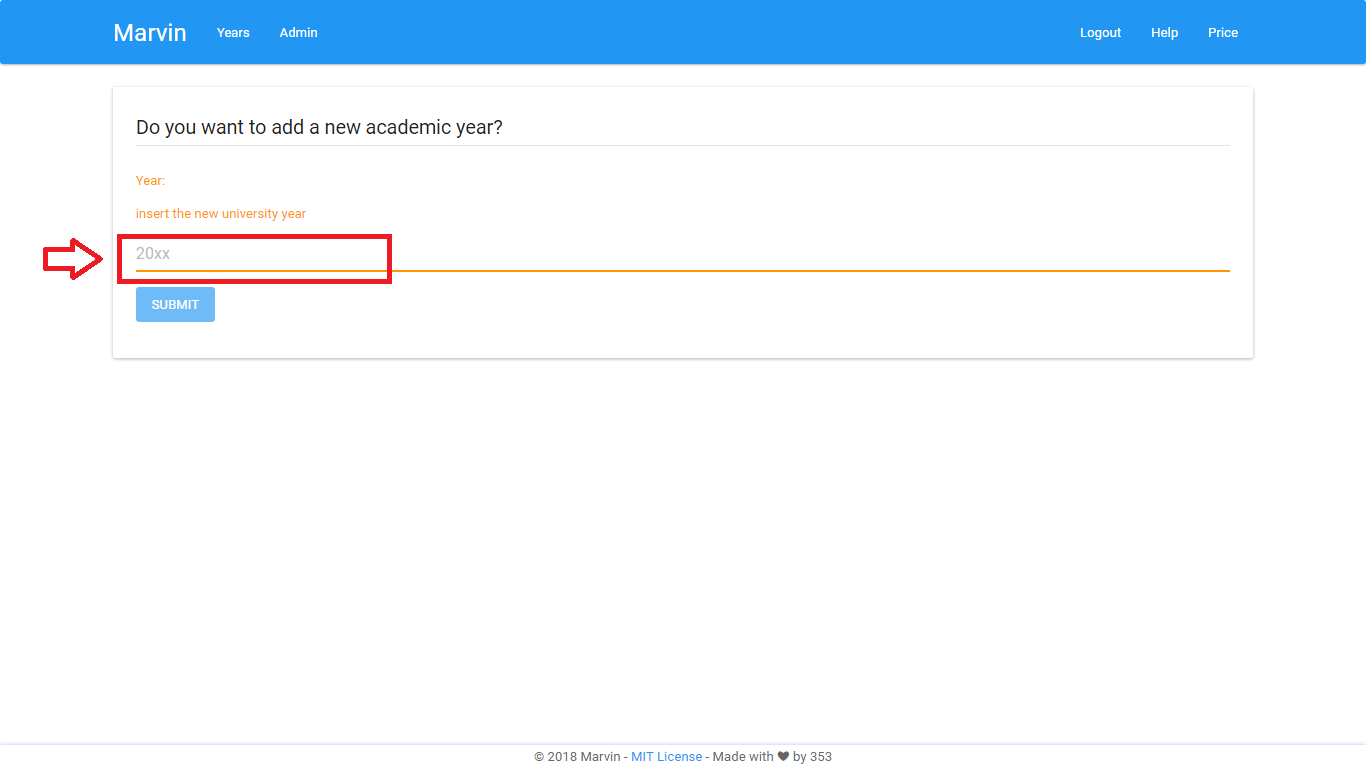
\includegraphics[width=0.7\linewidth]{image/UniversityAddYear1}
			\caption[Add year form]{Fill the form}
			\label{fig:Add a new academic year, fill the form}
		\end{figure}
		\item And then click the button ``SUBMIT".
		\begin{figure}[H]
			\centering
			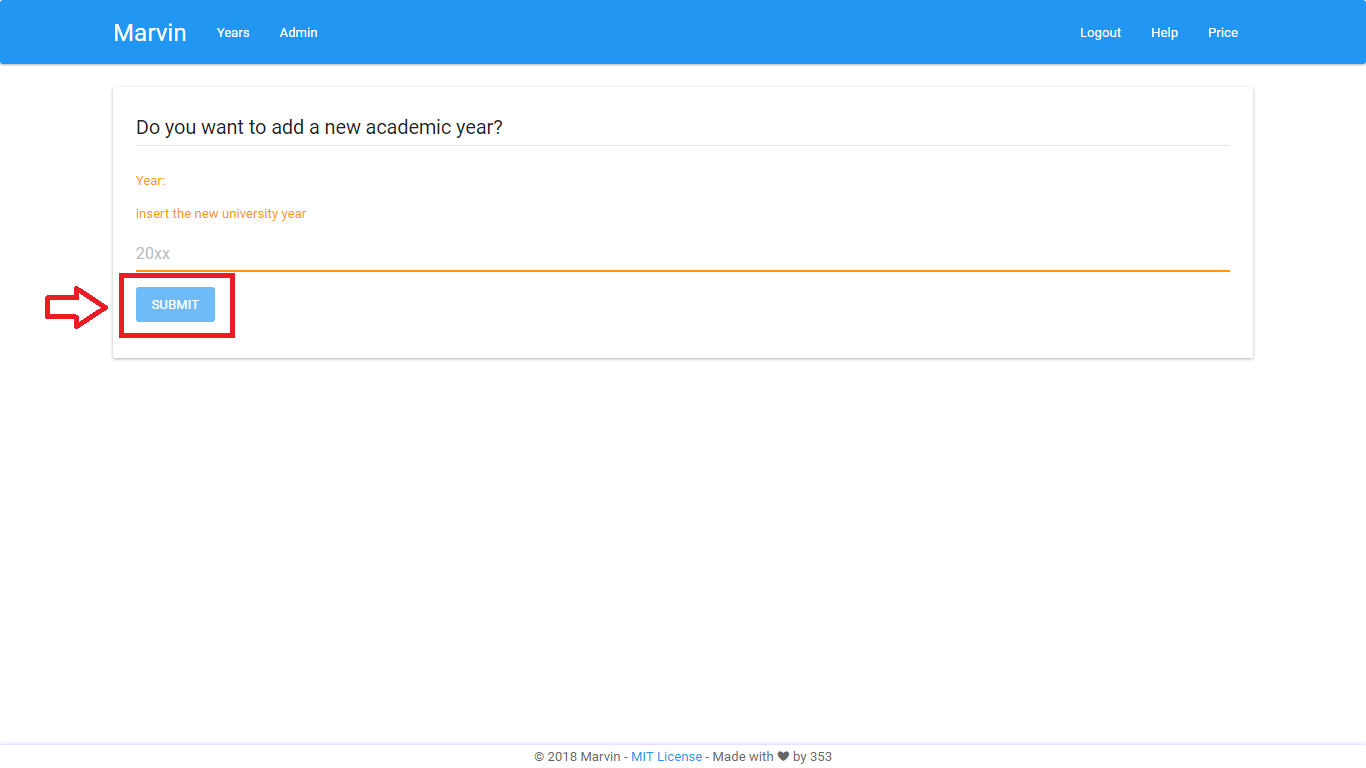
\includegraphics[width=0.7\linewidth]{image/UniversityAddYear2}
			\caption[Add year submit]{Click submit}
			\label{fig:Add a new academic year, click submit}
		\end{figure}
	\end{enumerate}

\subsection{Remove an academic year}
Only the academic years that do not contain courses can be removed, the attempt to remove an academic year containing at least one course will be reported as incorrect by Metamask.\\
To remove an academic year, you must go to the manage academic years section and click the "DELETE" button next to the year you want to delete.
\begin{figure}[H]
	\centering
	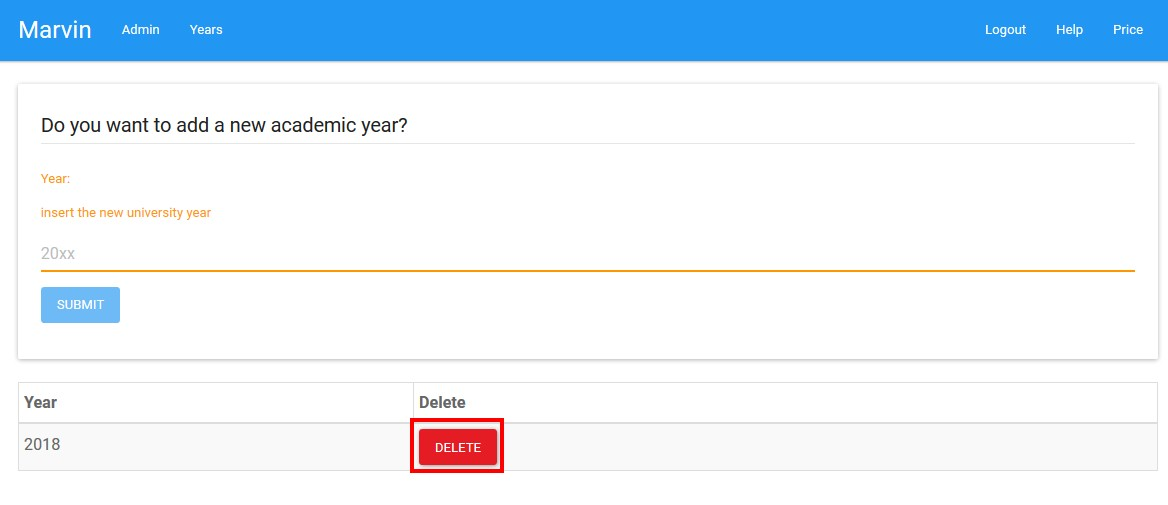
\includegraphics[width=0.7\linewidth]{image/UniversityRemoveYear1}
	\caption[Add year form]{Remove the year}
	\label{fig:Remove the year}
\end{figure}

\end{document}